% Provenance (never printed): see sources/outline_sources.md (Year 3:
% spectral signatures; optical, thermal and radar sensors; radar
% interferometry; digital elevation models; GIS operations).
% Brief: sources/book5/BRIEFS.md, ch. 25. Curves from figdata/bachelor-3/
% spectral_signatures.py (ECOSTRESS spectra and the Landsat 8 OLI bands),
% thermal_ir.py (Planck's law, brightness temperatures, a mixed pixel),
% insar_mogi.py (the wrapped interferogram of a Mogi source) and
% varden_gis.py (slope, aspect and an overlay on the Varden Hills, from
% figdata/shared/region.py, read only). Exercise and problem values in the
% Book 5 scratch calculator calc/ch25.py. Mount Halvren, its lava flows and
% its fumaroles are invented. The brief's overlay (slope > 15 degrees on
% limestone within 200 m of the river) is empty on the Varden model: the
% valley floor is flat; the printed overlay uses the shale within 1 km.
\chapter{الاستشعار عن بُعد ونظم المعلومات الجغرافية}\label{ch:b3:remote-sensing-gis}

في عام 1997 بدأت أرض منطقة برّية في سلسلة كاسكيد، قرب مجموعة
البراكين المسمّاة الأخوات الثلاث، بدأت في الارتفاع. وبحلول عام 2001 بات مركزها
أعلى بمقدار \qty{15}{cm}. لا يوجد بركان يعلو الانتفاخ مباشرةً، وآخر
ثوران في المنطقة قبل 1,500 سنة. ولم يلحظ الرفعَ
أحدٌ يسير فوقه، بل ظهر كهدف من حلقات ملوّنة عندما
دُمجت صور رادارية للمنطقة، التُقطت من المدار بفارق سنوات.
وحدّدت الحلقات عمق الصهارة المتسلّلة بين 6 و\qty{7}{km}؛ وفي مارس 2004
حدثت سلسلة من أكثر من 300 هزّة أرضية صغيرة قرب مركزها.
يشرح هذا الفصل كيف يقيس القمر الصناعي تغيّرًا لا يتجاوز بضعة
سنتيمترات من ارتفاع مئات الكيلومترات، وما تراه المستشعرات الأخرى في المدار
من الأرض، وكيف تُدمج الخرائط التي تُنتجها في نظام
المعلومات الجغرافية.
% ledger: usgs:insar-fs

\begin{recall}
الطيف الكهرومغناطيسي، وقانون بلانك للجسم الأسود، والانبعاثية
وقانون كيرشوف، والانعكاسية، وتداخل الموجات، موجودة في
كتب الفيزياء. الاستشعار عن بُعد، والصور الفضائية، وإسقاطات الخرائط،
وتحديد المواقع بالأقمار الصناعية موجودة في الكتب المدرسية. النوافذ الجوية
والنطاقات الضوئية موجودة في مجلد السنة الأولى، في فصله عن التلسكوبات؛
نموذج الارتفاع الرقمي ونظام المعلومات الجغرافية الذي
يخزّنه، في فصله عن الخرائط الجيولوجية؛ وأوّل خريطة رادارية
لإزاحة زلزال، في فصله عن مصدر الزلزال. ومصدر موغي
لخزان صهارة متضخّم موجود في مجلد السنة الثانية، في فصله عن
الثورات البركانية.
\end{recall}

\section{البصمات الطيفية والمستشعرات البصرية}\label{sec:b3:remote-sensing-gis:optical}

يُمتصّ جزء من ضوء الشمس الذي يصل إلى الأرض، ويُعكس جزء آخر،
بنسب تتوقّف على طول الموجة وعلى نوع المادة التي تتكوّن منها
الأرض. يقيس المستشعر في المدار الضوء المنعكس في عدد من مجالات طول
الموجة، أي نطاقاتها، وتحدّد النسب بينها
هويّة السطح.

\begin{definition}[البصمة الطيفية]\label{def:b3:remote-sensing-gis:signature}
\emph{البصمة الطيفية}\index{البصمة الطيفية} للمادة هي
انعكاسيّته بدلالة طول الموجة، $R(\lambda)$، أي نسبة
الإشعاع الساقط الذي تعكسه. وفي الأشعة تحت الحمراء الحرارية، حيث
تُصدر الأسطح الإشعاع بدلًا من أن تعكسه، تكون البصمة هي الانبعاثية
$\varepsilon(\lambda)$؛ وبالنسبة إلى عيّنة معتمة $\varepsilon = 1 - R$.
\end{definition}

\begin{omfigure}
\centering
\begin{tikzpicture}
\begin{axis}[width=0.9\linewidth, height=6.4cm, xmin=0.4, xmax=2.5, ymin=0, ymax=1,
  xlabel={طول الموجة \babelsublr{(\unit{\micro\metre})}}, ylabel={الانعكاسية},
  tick label style={font=\scriptsize}, label style={font=\small},
  legend style={font=\scriptsize, at={(0.5,-0.24)}, anchor=north, /tikz/every even column/.append style={column sep=4pt}},
  legend columns=5, clip=false]
\fill[black!8] (axis cs:0.45,0) rectangle (axis cs:0.51,1);
\fill[black!8] (axis cs:0.53,0) rectangle (axis cs:0.59,1);
\fill[black!8] (axis cs:0.64,0) rectangle (axis cs:0.67,1);
\fill[black!8] (axis cs:0.85,0) rectangle (axis cs:0.88,1);
\fill[black!8] (axis cs:1.57,0) rectangle (axis cs:1.65,1);
\fill[black!8] (axis cs:2.11,0) rectangle (axis cs:2.29,1);
\addplot[very thick, green!50!black] table[x=um, y=grass] {figdata/out/bachelor-3-spectral_signatures-spectra.dat};
\addlegendentry{عشب أخضر}
\addplot[thick, brown!70!black, dashed] table[x=um, y=soil] {figdata/out/bachelor-3-spectral_signatures-spectra.dat};
\addlegendentry{تربة رملية بنّية}
\addplot[thick, black!55] table[x=um, y=kaol] {figdata/out/bachelor-3-spectral_signatures-spectra.dat};
\addlegendentry{كاولينيت}
\addplot[thick, red!70!black, dash dot] table[x=um, y=hem] {figdata/out/bachelor-3-spectral_signatures-spectra.dat};
\addlegendentry{هيماتيت}
\addplot[thick, omDef] table[x=um, y=water] {figdata/out/bachelor-3-spectral_signatures-spectra.dat};
\addlegendentry{الماء}
\node[font=\tiny, anchor=south] at (axis cs:0.48,1) {2};
\node[font=\tiny, anchor=south] at (axis cs:0.56,1) {3};
\node[font=\tiny, anchor=south] at (axis cs:0.655,1) {4};
\node[font=\tiny, anchor=south] at (axis cs:0.865,1) {5};
\node[font=\tiny, anchor=south] at (axis cs:1.61,1) {6};
\node[font=\tiny, anchor=south] at (axis cs:2.2,1) {7};
\end{axis}
\end{tikzpicture}
\par\smallskip{\small أطياف الانعكاسية المخبرية لخمسة أسطح، من مكتبة
\babelsublr{ECOSTRESS Spectral Library}، أُعيد نشرها بإذن من مختبر دفع النفاثات
في معهد كاليفورنيا للتقنية، مع النطاقات الانعكاسية الستة
من 2 إلى 7 لمستشعري لاندسات~8 ولاندسات~9 المظلَّلةً. العشب الأخضر داكن في
المرئي، وأكثر سطوعًا في الأشعة تحت الحمراء القريبة؛ والكاولينيت ساطع في كل مكان
إلّا عند امتصاص ضيّق عند \qty{2.2}{\micro\metre}؛ والهيماتيت يمتصّ
الأزرق والأخضر ويعكس الأحمر؛ والماء يعكس بضعة بالمئة عند
كل طول موجة.}\label{fig:b3:remote-sensing-gis:spectra}
\end{omfigure}
% ledger: data:b5-ecostress, usgs:landsat8-bands, nasa:ndvi

البصمات الطيفية في الشكل أعلاه هي مفردات الاستشعار البصري عن بُعد
الكلوروفيل في الأوراق يمتصّ بقوّة بين 0.4
و\qty{0.7}{\micro\metre}، لأغراض التمثيل الضوئي، بينما تعكس خلايا الأوراق
بقوّة بين 0.7 و\qty{1.1}{\micro\metre}: يعكس العشب الأخضر
\qty{5}{\percent} من الضوء الأحمر للنطاق~4 و\qty{50}{\percent}
من الأشعة تحت الحمراء القريبة في النطاق~5، وهي قفزة لا تُحدثها أي صخرة أو تربة. وفيما بعد، يظهر
انخفاضان عميقان قرب 1.4 و\qty{1.9}{\micro\metre} حيث يمتصّ الماء السائل.
يزداد سطوع الرمل البنّي باطّراد نحو الأشعة تحت الحمراء. والكاولينيت،
وهو طين، أبيض في المرئي، ويمتلك امتصاصًا ضيّقًا عند
\qty{2.20}{\micro\metre}، داخل النطاق~7، مما يجعله أغمق هناك من
النطاق~6؛ ويستطيع \omterm{def:b3:remote-sensing-gis:sensors}{المستشعر فائق الطيفية} تحديد شكله والتمييز بين طين
وآخر. والهيماتيت يمتصّ الأزرق والأخضر، ومن هنا لونه الأحمر.
% ledger: nasa:ndvi, data:b5-ecostress

\begin{definition}[الاستبانة المكانية والطيفية والإشعاعية؛ زمن إعادة الزيارة]\label{def:b3:remote-sensing-gis:resolutions}
\emph{الاستبانة المكانية}\index{الاستبانة المكانية} لصورةٍ ما هي حجمُ
ما يغطّيه على الأرض أحدُ بكسلاتها. أمّا \emph{الاستبانة
الطيفية}\index{الاستبانة الطيفية} هي عددُ حزمها وعرضُ كلٍّ منها،
أمّا \emph{الاستبانة الإشعاعية}\index{الاستبانة الإشعاعية} فهي
عددُ المستويات التي يُسجَّل فيها كلُّ قياس، أي $2^b$ مستوى عند $b$ بت.
أمّا \emph{زمن إعادة الزيارة}\index{زمن إعادة الزيارة} لقمرٍ صناعي فهو الفترة
الزمنية الفاصلة بين رصدين له لمكانٍ واحد.
\end{definition}

لا يمكن أن تكون الأربعة دقيقةً معًا: فالبكسلات الأصغر والحزم الأضيق
تجمع كلٌّ منها ضوءًا أقلّ، ويستغرق شريطٌ ضيّق وقتًا أطول لتغطية
الأرض. يحمل الماسح الضوئي للقمر لاندسات~8، الذي أُطلق عام 2013، تسع حزم، أغلبها
منها بكسلات \qty{30}{m} وحزمةٌ واحدة بانكروماتية عند \qty{15}{m}؛ وتسجّل
4096 مستوى (12 بت)، في حين سجّلت أجهزة لاندسات 1 إلى 7
تسجّل 256. ومن مدار متزامن مع الشمس على ارتفاع \qty{705}{km} يصوّر
شريطًا عرضه \qty{185}{km} ويعود إلى المكان نفسه كلّ 16 يومًا؛
لاندسات~9، الذي يدور في المدار نفسه بفارق 8 أيام، يُنصّف زمن الانتظار.
يحمل الماسح الضوئي متعدّد الأطياف لكلّ قمر سنتينل-2 13 حزمةً، بكسلاتٍ قدرها 10 أو 20
أو \qty{60}{m}، على شريط عرضه \qty{290}{km}؛ ومع قمرين في المدار نفسه يكون
\omterm{def:b3:remote-sensing-gis:resolutions}{زمن إعادة الزيارة} عند خطّ الاستواء 5 أيام.
% ledger: usgs:landsat8-bands, usgs:landsat8-orbit, esa:s2-msi, esa:s2-orbit

\begin{definition}[المستشعرات متعدّدة الأطياف وفائقة الطيفية]\label{def:b3:remote-sensing-gis:sensors}
يسجّل \emph{المستشعر متعدّد الأطياف}\index{المستشعر متعدّد الأطياف} عددًا قليلًا
إلى بضعة عشرات من الحزم، تفصل بينها فجوات. أمّا \emph{المستشعر فائق
الطيفية}\index{المستشعر فائق الطيفية} يسجّل حزمًا كثيرةً ضيّقةً متلاصقة،
بحيث يحمل كلّ بكسل طيفًا شبه متصل يمكن مقارنته
بمكتبةٍ كالتي في الشكل أعلاه.
\end{definition}

يقع الغلاف الجوي بين الأرض والمستشعر. ويبعثر
ضوء الشمس نحو المستشعر، وهو ضوءٌ لم يلامس الأرض قطّ، وذلك أكثر ما يكون عند
الأطوال الموجية القصيرة، ويُسمّى هذا الإشعاع إشعاعَ المسار، ويمتصّ جزءًا مما
تعكسه الأرض خارج النوافذ الجوية.

\begin{definition}[التصحيح الجوي]\label{def:b3:remote-sensing-gis:atm-correction}
\emph{التصحيح الجوي}\index{التصحيح الجوي} هو
تحويل الإشعاع المقاس عند أعلى الغلاف الجوي إلى
انعكاسية السطح، بإزالة إشعاع المسار وتعويض
الامتصاص على مساري الضوء، الهابط والصاعد.
\end{definition}

أبسط التصحيحات يطرح في كلّ حزمة قيمة أغمق
البكسلات في المشهد، كالماء الصافي العميق أو الظلّ، والتي ينبغي ألّا تعكس
شيئًا تقريبًا، فما تُظهره هو إشعاع المسار. وتنمذج التصحيحات الدقيقة
جزيئات الغلاف الجوي والهباء الجوي وبخار الماء.

\begin{definition}[مؤشّر الغطاء النباتي للفرق المعياري]\label{def:b3:remote-sensing-gis:ndvi}
يُعرَّف \emph{مؤشّر الغطاء النباتي للفرق
المعياري}\index{مؤشّر الغطاء النباتي للفرق المعياري} (NDVI) لبكسلٍ ما هو:
\[
\mathrm{NDVI} = \frac{R_\mathrm{NIR} - R_\mathrm{red}}{R_\mathrm{NIR} + R_\mathrm{red}} ,
\]
تُحسب من انعكاسيّته في حزمة تحت الحمراء القريبة وحزمة حمراء.
\end{definition}

يقع المؤشّر بين $-1$ و$+1$. ويعطي سطحٌ خالٍ من أوراق خضراء
قيمةً قريبةً من الصفر، كالصخر العاري والرمل والثلج، بقيمة \num{0.1} فأدنى،
الشجيرات والمراعي 0.2 إلى 0.3، والغابات المطرية المعتدلة والاستوائية 0.6 إلى
0.8؛ وتقترب أكثف الأوراق الخضراء من 0.8 إلى 0.9. ومن أطياف الشكل
أعلاه، عبر النطاقين 4 و5، يعطي العشب 0.82، والرمل البنّي
0.15، والماء $-0.01$. ولأنّ المؤشّر نسبةٌ، فإنّه لا يتغيّر حين
يخفت النطاقان بالنسبة نفسها، كأن يكون ذلك بسبب منحدر يواجه بعيدًا عن
الضوء أو ضبابٍ خفيفٍ متجانس: إنّه يقيس الغطاء النباتي لا
الإضاءة. أمّا إشعاع المسار المضاف، وهو أكبر في الأحمر، فيغيّره،
ولهذا يُحسب المؤشّر من الانعكاسيّات المصحّحة
(انظر \cref{exo:b3:remote-sensing-gis:12}).
% ledger: nasa:ndvi, data:b5-ecostress

\section{الأشعة تحت الحمراء الحرارية}\label{sec:b3:remote-sensing-gis:thermal}

عند درجات حرارة الأرض، نحو \qty{300}{K}، يضع قانون بلانك
ذروةَ انبعاث الجسم الأسود قرب \qty{9.7}{\micro\metre}، في
نافذة الغلاف الجوي للأشعة تحت الحمراء الحرارية. وهناك يقيس المستشعر ما
يبعثه السطح، لا ما يعكسه. ويملك المستشعر الحراري للقمر لاندسات~8
حزمتين، من 10.6 إلى 11.19 ومن 11.5 إلى \qty{12.51}{\micro\metre}، وبكسلاتهما
بكسلاتٍ قياسها \qty{100}{m}.
% ledger: const:h, const:c, const:kB, usgs:landsat8-bands

\begin{definition}[درجة حرارة السطوع]\label{def:b3:remote-sensing-gis:brightness}
\emph{درجة حرارة السطوع}\index{درجة حرارة السطوع} $T_b$ لسطحٍ
عند الطول الموجي $\lambda$ هي درجة حرارة الجسم الأسود
الذي يبعث الإشعاع الطيفي $L$ المقاس منه عند ذلك
الطول الموجي. أمّا \emph{درجة الحرارة الحركية} فهي درجة الحرارة الديناميكية الحرارية للسطح،
أي تلك التي يقرؤها مقياس الحرارة.
\end{definition}

\begin{proposition}[درجة حرارة السطوع انطلاقًا من الإشعاع]\label{prop:b3:remote-sensing-gis:planck-inversion}
مع $c_1 = 2hc^2$ و$c_2 = hc/k$، فإنّ الإشعاع الطيفي $L$ عند
الطول الموجي $\lambda$ له \omterm{def:b3:remote-sensing-gis:brightness}{درجة حرارة السطوع}
\[
T_b = \frac{c_2}{\lambda \ln\!\left(1 + \dfrac{c_1}{\lambda^5 L}\right)} .
\]
سطحٌ ذو انبعاثية $\varepsilon < 1$ عند درجة الحرارة الحركية $T$
يبعث $L = \varepsilon B_\lambda(T)$ ويكون له $T_b < T$.
\end{proposition}

\begin{proof}
يعطي قانون بلانك $B_\lambda(T) = c_1\lambda^{-5}/(e^{c_2/\lambda T} -
1)$. بوضع $B_\lambda(T_b) = L$ وحلّ المعادلة، $e^{c_2/\lambda T_b} = 1 +
c_1/(\lambda^5L)$، وهو الصيغة المطلوبة. يتزايد $B_\lambda$ مع
درجة الحرارة، لذا فإنّ $\varepsilon B_\lambda(T) < B_\lambda(T)$ يستلزم $T_b < T$.
\end{proof}
% ledger: const:h, const:c, const:kB

للفرق أهميّة. ففي مركز النطاق~10، \qty{10.9}{\micro\metre}،
يكون سطحٌ عند \qty{300}{K} ذو انبعاثية 0.95 درجةَ سطوع
قدرها \qty{296.6}{K}، وقدرها \qty{299.3}{K} عند انبعاثية 0.99: يُساوي واحدٌ في المئة من
الانبعاثية أكثرَ من نصف كلفن. وتعطي الأطياف المخبرية،
في النطاق~10 انبعاثية قدرها 0.98 للعشب، و0.99 للماء،
و0.97 للرمل البنّي. ولذلك يحتاج رسم درجة الحرارة من المدار إلى
انبعاثية كلّ بكسل، وإلى تصحيحٍ للانبعاث وامتصاص الهواء
الفاصل بينهما.
% ledger: data:b5-ecostress

\begin{omfigure}
\centering
\begin{tikzpicture}
\begin{groupplot}[group style={group size=2 by 1, horizontal sep=1.5cm},
  width=0.48\linewidth, height=0.42\linewidth,
  tick label style={font=\scriptsize}, label style={font=\small}, title style={font=\small}]
\nextgroupplot[title={إشعاع الجسم الأسود}, xmode=log, ymode=log, xmin=1, xmax=25,
  ymin=0.01, ymax=1e5, xlabel={الطول الموجي \babelsublr{(\unit{\micro\metre})}},
  ylabel={\mbox{\textdir TLT $B_\lambda$ (\unit{W.m^{-2}.sr^{-1}.\micro\metre^{-1}})}},
  xtick={1,2,5,10,20}, xticklabels={1,2,5,10,20}]
\fill[black!10] (axis cs:10.6,0.01) rectangle (axis cs:11.19,1e5);
\fill[black!10] (axis cs:2.11,0.01) rectangle (axis cs:2.29,1e5);
\addplot[thick, omDef] table[x=um, y=b300] {figdata/out/bachelor-3-thermal_ir-planck.dat};
\addplot[thick, omDef, dashed] table[x=um, y=b400] {figdata/out/bachelor-3-thermal_ir-planck.dat};
\addplot[thick, red!70!black] table[x=um, y=b1443] {figdata/out/bachelor-3-thermal_ir-planck.dat};
\node[font=\scriptsize, omDef, anchor=north east] at (axis cs:24,3) {\qty{300}{K}};
\node[font=\scriptsize, omDef, anchor=south west] at (axis cs:12.5,30) {\qty{400}{K}};
\node[font=\scriptsize, red!70!black, anchor=south west] at (axis cs:3.2,2000) {\qty{1443}{K}};
\node[font=\tiny, anchor=north] at (axis cs:10.9,1e5) {10};
\node[font=\tiny, anchor=north] at (axis cs:2.2,1e5) {7};
\nextgroupplot[title={بكسل مختلط، النطاق 10}, xmin=0, xmax=1, ymin=285, ymax=375,
  xlabel={نسبة $f$ من البكسل عند \qty{370}{K}}, ylabel={درجة الحرارة \babelsublr{(\unit{K})}},
  legend style={font=\scriptsize, at={(0.97,0.03)}, anchor=south east}]
\addplot[thick, red!70!black] table[x=f, y=tb] {figdata/out/bachelor-3-thermal_ir-mixed.dat};
\addlegendentry{درجة حرارة السطوع}
\addplot[thick, black!60, dashed, domain=0:1] {290 + 80*x};
\addlegendentry{متوسط درجة الحرارة}
\end{groupplot}
\end{tikzpicture}
\par\smallskip{\small يسارًا، قانون بلانك للأسطح عند 300 و\qty{400}{K}
وللحمم الناتجة عن ثوران عند \qty{1170}{\celsius} (\qty{1443}{K})، مع
نطاق الأشعة تحت الحمراء القصيرة~7 والنطاق الحراري~10 من لاندسات~8 مظلَّلان.
يمينًا، \omterm{def:b3:remote-sensing-gis:brightness}{درجة حرارة السطوع} في النطاق~10 لبكسل تكون فيه نسبة
$f$ منه عند \qty{370}{K} والباقي عند \qty{290}{K}، مقارنةً
بمتوسط درجة الحرارة المرجَّح بالمساحة: الجزء الحار يُحسب أكثر من
مساحته.}\label{fig:b3:remote-sensing-gis:thermal}
\end{omfigure}
% ledger: const:h, const:c, const:kB, usgs:landsat8-bands, usgs:kilauea-temp

للحمم عند \qty{1170}{\celsius} ذروةٌ قرب \qty{2.0}{\micro\metre}: فتدفّقُ
حممٍ حديثٌ أصغرُ بكثير من البكسل يُضيء نطاقات الأشعة تحت الحمراء القصيرة
في مُصوِّرٍ بصريّ، نهارًا أو ليلًا. البكسل نادرًا ما يكون متجانسًا،
وقانونُ بلانك ليس خطيًّا في درجة الحرارة.
% ledger: usgs:kilauea-temp

\begin{proposition}[بكسل مختلط]\label{prop:b3:remote-sensing-gis:mixed}
بكسلٌ تُشعّ منه نسبةٌ $f$ كجسمٍ أسود عند $T_h$، والباقي
عند $T_0 < T_h$ تكون له شدةُ الإشعاع $L = fB_\lambda(T_h) + (1 - f)B_\lambda(T_0)$،
ومن أجل $0 < f < 1$، تتجاوز درجة حرارة سطوعه متوسطَ درجة الحرارة المرجَّح
بالمساحة $fT_h + (1 - f)T_0$.
\end{proposition}

\begin{proof}
شدّة الإشعاع هي متوسطُ شدّات الإشعاع المرجَّحُ بالمساحة. نكتب $B_\lambda(T)
= c_1\lambda^{-5}g(c_2/\lambda T)$ حيث $g(x) = 1/(e^x - 1)$؛ في
المتغيّر $T$، مع $x = c_2/\lambda T$، فإنّ المشتقّة الثانية للدالة
$g(c_2/\lambda T)$ هي $(x g''(x) + 2g'(x))\,x/T^2$، موجبةٌ عندما $x(e^x + 1)
> 2(e^x - 1)$، أي $x > 2\tanh(x/2)$، وهذا متحقّق من أجل كلّ $x > 0$:
$B_\lambda$ محدّبةٌ في $T$. وبحكم التحدّب
يتجاوز متوسط الإشعاعات إشعاعَ متوسطِ درجة الحرارة،
و$B_\lambda$ يتزايد مع $T$، فإنّ $T_b > fT_h + (1 - f)T_0$.
\end{proof}

بكسلٌ فيه \qty{5}{\percent} من
أرضُ الفومارول عند \qty{370}{K} في خلفيّةٍ عند \qty{290}{K} لها متوسطُ
درجةِ حرارةٍ \qty{294}{K}، لكنّ درجةَ حرارة سطوعها \qty{295.3}{K}؛ وعند
\qty{10}{\percent}، \qty{300.4}{K}. تبرز البقع الساخنة في صورة حرارية،
ولا يمكن قراءة درجة حرارتها من نطاق واحد وحده: فنطاقان
مختلفا الطول الموجي يُعطيان معادلتين بالمجهولين $f$ و$T_h$.

\section{الرادار والليدار}\label{sec:b3:remote-sensing-gis:radar}

المستشعر البصري أو الحراري سلبيٌّ: يقيس الضوء الذي تُرسله الأرض
أمّا الرادار أو \omterm{def:b3:remote-sensing-gis:lidar}{الليدار} فنشِط: يُرسل نبضةً ويقيس زمن صداها.
تنفذ الموجات الدقيقة عبر الغيوم، ويوفّر الرادار إضاءته الخاصة،
فيرصد نهارًا وليلًا وفي أيّ طقس.
% ledger: esa:s1-sar

\begin{definition}[رادار الفتحة الاصطناعية؛ التشتّت الخلفي للرادار]\label{def:b3:remote-sensing-gis:sar}
\emph{رادار الفتحة الاصطناعية}\index{رادار الفتحة الاصطناعية} \babelsublr{(SAR)} هو
رادارٌ يُحمَل على مسارٍ يرصد جانبيًّا، ويدمج الأصداء التي يسجّلها من
النقطةِ نفسها من الأرض على امتداد طولٍ من مساره، محافظًا على أطوارها،
كأنّها استُقبلت بهوائيٍّ واحد بطول ذلك الطول.
أمّا \emph{التشتّت الخلفي للرادار}\index{التشتّت الخلفي للرادار} لسطحٍ فهو
نسبةُ القدرة المستقبَلة التي يُعيدها
نحو الهوائي.
\end{definition}

\begin{omfigure}
\centering
\begin{tikzpicture}[>=stealth, font=\small, x=1cm, y=1cm]
\fill[black!12] (-0.5,-0.35) rectangle (10.5,0);
\draw[thick] (-0.5,0) -- (10.5,0);
% satellite
\fill[omDef] (0.6,4.6) rectangle (1.4,5.0);
\draw[thick, omDef] (0.35,4.45) -- (1.65,5.15);
\draw (1.0,4.8) circle (0.12); \fill (1.0,4.8) circle (0.03);
 \node[font=\scriptsize, anchor=south, align=center] at (1.0,5.3) {\foreignlanguage{arabic}{الطيران (السمت)}\\داخل الصفحة};
% nadir
\draw[dashed, black!60] (1.0,4.4) -- (1.0,0);
\node[font=\scriptsize, anchor=north] at (1.0,-0.4) {النادير};
\draw[<->, black!60] (0.3,0) -- node[left, font=\scriptsize] {$h$} (0.3,4.4);
% beam
\fill[omDef!12] (1.0,4.4) -- (4.3,0) -- (9.6,0) -- cycle;
\draw[omDef!60] (1.0,4.4) -- (4.3,0); \draw[omDef!60] (1.0,4.4) -- (9.6,0);
\node[font=\scriptsize, anchor=north] at (4.3,-0.4) {المدى القريب};
\node[font=\scriptsize, anchor=north] at (9.6,-0.4) {المدى البعيد};
\draw[<->] (4.3,-1.0) -- node[below, font=\scriptsize] {الشريط الماسح} (9.6,-1.0);
% target and slant range
\fill[red!70!black] (7.0,0) circle (0.07);
\draw[thick, red!70!black] (1.0,4.4) -- node[above, sloped, font=\scriptsize] {\foreignlanguage{arabic}{المدى المائل $R$}} (7.0,0);
\draw[black!60] (7.0,0) -- (7.0,1.8);
\draw[black!60] (7.0,0.9) arc (90:126.25:0.9);
\node[font=\scriptsize] at (6.6,1.2) {$\theta$};
\draw[->, very thick, omThm] (7.0,0) -- (6.2,0.59) node[anchor=north east, font=\scriptsize, inner sep=1pt] {LOS};
\draw[<->, black!60] (1.0,-1.6) -- node[below, font=\scriptsize] {المدى الأرضي} (7.0,-1.6);
\draw[black!60] (1.0,-1.5) -- (1.0,-1.7); \draw[black!60] (7.0,-1.5) -- (7.0,-1.7);
\end{tikzpicture}
\par\smallskip{\small هندسةُ رادارٍ جانبيّ النظر، في المستوى
العمودي على مساره. يُضيء الشعاعُ الشريطَ الماسحَ إلى أحد جانبَي
النادير؛ تُرى نقطةٌ من الأرض عند المدى المائل $R$ تحت
زاوية السقوط $\theta$، على طول \omterm{def:b3:remote-sensing-gis:insar}{خط النظر} \babelsublr{(LOS)}. تُرتَّب الأصداء
بحسب تأخّرها عبر المسار، أي في المدى، وبحسب تاريخ
الطور للفتحة الاصطناعية على امتدادها، أي في السمت.}\label{fig:b3:remote-sensing-gis:sar}
\end{omfigure}

\begin{proposition}[الاستبانة السمتية]\label{prop:b3:remote-sensing-gis:azimuth}
لا يميّز هوائي حقيقي طوله $L$ عند المدى المائل $R$ نقطتين من سطح الأرض
على امتداد مساره، إلّا إذا كانتا تبعدان أكثر من نحو $R\lambda/L$
عن بعضهما. ويبلغ \omterm{def:b3:remote-sensing-gis:sar}{رادار الفتحة الاصطناعية} بالهوائي نفسه نحو $L/2$
مهما كان المدى.
\end{proposition}

\begin{proof}
ينتشر شعاع الهوائي الذي طوله $L$ عبر زاوية تبلغ نحو
$\lambda/L$، فيضيء شريطًا طوله $R\lambda/L$ على امتداد المسار، ولا
يستطيع الهوائي الحقيقي التمييز بين نقطتين داخله. وتبقى النقطة في
الشعاع ما دام الهوائي يقطع الطول نفسه $\ell = R\lambda/L$:
وهذا هو مفهوم الفتحة الاصطناعية. ويكافئ جمع الأصداء على امتداد $\ell$
هوائيًا طوله $\ell$؛ ويُقطع مسار كل صدى
مرّتين، ذهابًا وإيابًا، وهذا يُنصّف شعاع الهوائي الاصطناعي
ليصبح $\lambda/(2\ell)$، وتكون الاستبانة $R\lambda/(2\ell) =
L/2$. وتبقى النقطة الأبعد مدّة أطول في الشعاع، فالفتحة الأطول
تعوّض تمامًا المدى الأكبر.
\end{proof}

يعمل رادار كل قمر من أقمار سنتينل-1 في نطاق C، عند
\qty{5.405}{GHz}، وطول موجة نحو \qty{5.55}{cm}، وبهوائي
طوله \qty{12.3}{m}، من ارتفاع \qty{693}{km}. ولا يميّز هوائي حقيقي بهذا الحجم
تفاصيل أدقّ من نحو \qty{4}{km} على امتداد المسار، بينما تُنزل الفتحة الاصطناعية
قيمة $L/2$ إلى نحو \qty{6}{m}. ويعمل فوق اليابسة غالبًا في
نمط الشريط العريض الذي يمسح ثلاثة أشرطة فرعية لتغطية \qty{250}{km}، بزوايا سقوط
بين 29 و\ang{46}، بأبعاد 5 في \qty{20}{m}.
يكرّر القمر الواحد مداره كل 12 يومًا.
% ledger: esa:s1-sar, esa:s1-orbit, esa:s1-iw

يعتمد \omterm{def:b3:remote-sensing-gis:sar}{التشتّت الخلفي للرادار} على خشونة السطح بمقياس
طول الموجة وعلى رطوبته. تعكس البحيرة الساكنة النبضة بعيدًا، كالمرآة،
فتبدو داكنة؛ أمّا تدفّق الحمم الخشن أو تاج الغابة أو مدينة ذات جدران
وزوايا فتعيد جزءًا كبيرًا منها وتبدو ساطعة.

\begin{definition}[الليدار]\label{def:b3:remote-sensing-gis:lidar}
\emph{الليدار}\index{الليدار} يقيس المسافات بزمن انتقال النبضات الليزرية
المرتدّة عن الأرض أو الغطاء النباتي أو الماء.
\end{definition}

\begin{proposition}[زمن الطيران]\label{prop:b3:remote-sensing-gis:tof}
نبضة تعود بعد زمن $t$ من انطلاقها قد لاقت سطحًا على المسافة
$ct/2$؛ وعدم اليقين $\delta t$ في الزمن هو عدم يقين
$c\,\delta t/2$ في المسافة.
\end{proposition}

\begin{proof}
يقطع الضوء بسرعة $c$ مسافة ذهابًا وإيابًا تساوي $2d = ct$.
\end{proof}

يطلق مقياس الارتفاع الليزري في آيس سات-2، من ارتفاع نحو \qty{500}{km}،
\num{10000} نبضة في الثانية عند \qty{532}{nm} عبر ستّ حزم، واحدة كل
\qty{0.7}{m} على امتداد الأرض ضمن بقعة قطرها \qty{11}{m}. ومن بين
نحو 300~تريليون فوتون تنطلق مع كل نبضة لا يعود منها إلا نحو اثني عشر
فوتونًا، ويُقاس زمن كل منها بدقّة \qty{800}{ps}، أي \qty{12}{cm} من المدى.
فوق الغابة تعود بعض الفوتونات من التاج وبعضها من الأرض
عبر فجواته؛ والفرق بينهما هو ارتفاع الأشجار، وفوتونات الأرض وحدها
تعطي خريطة للتضاريس تحتها. وترسم أجهزة \omterm{def:b3:remote-sensing-gis:lidar}{الليدار} المحمولة على
متن الطائرات الأرض تحت الغطاء النباتي بالطريقة نفسها.
% ledger: nasa:icesat2-atlas, nasa:icesat2-photons

\section{قياس التداخل الراداري}\label{sec:b3:remote-sensing-gis:insar}

يملك الصدى الذي يسجّله الرادار سعةً، أي قوّة العودة،
وطورًا يُحصي مسافة الذهاب والإياب بوحدات
طول الموجة. ولا يفيد طور صورة واحدة وحدها: إذ يحوي كل بكسل عددًا كبيرًا من المبعثرات
تتراكم أصداؤها بأطوار عشوائية. ولكن إن لم تتغيّر الأرض بين التقاطَين،
فإنّ المبعثرات نفسها تعطي المجموع نفسه مجددًا.
% ledger: usgs:insar-vhp

\begin{definition}[قياس التداخل الراداري؛ مخطط التداخل؛ خط النظر]\label{def:b3:remote-sensing-gis:insar}
\emph{قياس التداخل الراداري}\index{قياس التداخل الراداري} (InSAR) يجمع
صورتين راداريتين للأرض نفسها، التقطتا من موقع يكاد يكون واحدًا
في زمنين مختلفين، بكسلًا ببكسل. و\emph{مخطط التداخل}\index{مخطط التداخل}
هو خريطة لفرق طوريهما، المعلوم بترديد $2\pi$
والمرسوم دورةً من الألوان، وكل دورة \emph{هُدبة}. و\emph{خط
النظر}\index{خط النظر (الرادار)} هو الاتجاه من الأرض إلى
الهوائي؛ ولا يقيس الرادار إلا مركّبة الإزاحة على
امتداده. و\emph{فكّ التفاف الطور}\index{فكّ التفاف الطور} هو إعادة بناء
الطور المتصل من الطور الملتفّ، بإضافة إلى كل بكسل
مضاعف $2\pi$ الذي يجعل الطور يتغيّر بسلاسة عن جيرانه.
\end{definition}

\begin{theorem}[هدبة واحدة]\label{thm:b3:remote-sensing-gis:fringe}
بين تسجيلين متتاليين من الموقع نفسه، فإنّ إزاحة للأرض
التي تقصّر المسافة إلى الهوائي بمقدار $\Delta r$ تغيّر
طور صداها بمقدار $\Delta\phi = 4\pi\Delta r/\lambda$. والهدبة الواحدة، تغيّرٌ
مقداره $2\pi$، حركةٌ مقدارها $\lambda/2$ على طول \omterm{def:b3:remote-sensing-gis:insar}{خط النظر}.
\end{theorem}

\begin{proof}
يقطع الصدى المسافة $2r$ ذهابًا وإيابًا، ويكون طوره
$2\pi\cdot 2r/\lambda$ مضافًا إليه ثابت تحدّده المبعثرات، وهو نفسه في
الصورتين. والفرق هو $4\pi\Delta r/\lambda$، ويساوي $2\pi$
عندما يكون $\Delta r = \lambda/2$.
\end{proof}

بالنسبة إلى سنتينل-1 تبلغ الهدبة \qty{27.7}{mm}؛ أمّا الأقمار
الأوروبية والكندية الأقدم، ذات طول الموجة \qty{5.66}{cm}، فالهدبة \qty{28.3}{mm}، أي
دورة الألوان في الصورة أدناه. وعمليًا تختلف مواضع المرورين
بمقدار يصل إلى مئة متر تقريبًا (يُحفَظ القمر سنتينل-1
ضمن \qty{120}{m} من مدار مرجعي)، ويحوي فرق الطور أيضًا
التضاريس، وهذه يزيلها نموذج الارتفاع الرقمي؛
ويؤخّر بخار الماء في الغلاف الجوي الموجات بصورة مختلفة في التاريخين؛
وحيثما تتغيّر الأرض بين المرورين، وخاصةً الغطاء النباتي،
تفقد الأطوار ترابطها، فتذوب الهدب في الضجيج. أمّا طول الموجة
الأطول لنطاق L، \qty{23.53}{cm}، فيخترق الغطاء النباتي أفضل من
نطاق C.
% ledger: esa:s1-sar, esa:s1-orbit, usgs:insar-fs, photo:b3-three-sisters-insar

\begin{proposition}[مصدر موجي كما يُرى على طول خط النظر]\label{prop:b3:remote-sensing-gis:mogi-los}
فوق مصدر موجي لتغيّر الحجم $\Delta V$ على العمق $z_0$، وعلى المسافة
الأفقية $r$، ترتفع الأرض بمقدار $u_z$، كما في مجلد السنة الثانية،
وتتحرّك نحو الخارج بمقدار
\[
u_r = \frac{(1 - \nu)\,\Delta V}{\pi}\,\frac{r}{(r^2 + z_0^2)^{3/2}} = \frac{r}{z_0}\,u_z .
\]
عند زاوية السقوط $\theta$ من قمر صناعي واقع شرقًا، يكون تغيّر \omterm{def:b3:remote-sensing-gis:insar}{خط النظر}
هو $d = u_E\sin\theta + u_z\cos\theta$، و$u_E$ هي الإزاحة نحو الشرق.
على الخط الشمالي--الجنوبي المار بالمركز،
$d = u_z\cos\theta$.
\end{proposition}

\begin{proof}
الصيغة الشعاعية هي نظيرة الصيغة الرأسية في الحل
نفسه. المتجهة الواحدية الموجَّهة من الأرض نحو القمر الصناعي هي
$(\sin\theta, 0, \cos\theta)$ في اتجاهات الشرق والشمال والأعلى، ويكون تغيّر المسافة
هو سالب مسقط الإزاحة عليها، ومنه يكون التقصير
هو $d$. أمّا على الخط الشمالي--الجنوبي فالحركة الخارجية
شمالًا أو جنوبًا، عمودية على تلك المتجهة، و$u_E = 0$.
\end{proof}
% ledger: dmodels:mogi, dmodels:mogi-radial

\begin{omfigure}
\centering
\begin{tikzpicture}
\begin{groupplot}[group style={group size=2 by 1, horizontal sep=1.5cm},
  tick label style={font=\scriptsize}, label style={font=\small}, title style={font=\small}]
\nextgroupplot[title={مخطّط التداخل الملفوف}, width=0.46\linewidth, height=0.46\linewidth,
  axis equal image, enlargelimits=false, xmin=-15, xmax=15, ymin=-15, ymax=15,
  xlabel={الشرق \babelsublr{(\unit{km})}}, ylabel={الشمال \babelsublr{(\unit{km})}},
  colormap={fringe}{rgb255=(128,0,170) rgb255=(30,60,220) rgb255=(0,170,220) rgb255=(30,170,60) rgb255=(240,220,0) rgb255=(240,120,0) rgb255=(220,20,30) rgb255=(128,0,170)},
  point meta min=0, point meta max=6.2832]
\addplot[matrix plot*, mesh/cols=101, point meta=explicit] table[x=x, y=y, meta=phase] {figdata/out/bachelor-3-insar_mogi-map.dat};
\draw[->, very thick, white] (axis cs:6,-12.5) -- (axis cs:12,-12.5);
\node[font=\scriptsize, white, anchor=south] at (axis cs:9,-12.3) {نحو القمر الصناعي};
\nextgroupplot[title={المقاطع}, width=0.5\linewidth, height=0.46\linewidth,
  xmin=-15, xmax=15, ymin=-60, ymax=240, xlabel={المسافة عن المركز \babelsublr{(\unit{km})}},
  ylabel={الإزاحة \babelsublr{(\unit{mm})}}, legend columns=2,
  legend style={font=\scriptsize, at={(0.5,0.98)}, anchor=north, /tikz/every even column/.append style={column sep=4pt}}]
\addplot[thick, black] table[x=x, y=uz] {figdata/out/bachelor-3-insar_mogi-profile.dat};
\addlegendentry{$u_z$}
\addplot[thick, black!50, dashed] table[x=x, y=ue] {figdata/out/bachelor-3-insar_mogi-profile.dat};
\addlegendentry{$u_E$}
\addplot[very thick, red!70!black] table[x=x, y=los] {figdata/out/bachelor-3-insar_mogi-profile.dat};
\addlegendentry{\foreignlanguage{arabic}{\mbox{\textdir TLT LOS}، شرق--غرب}}
\addplot[thick, omDef, dash dot] table[x=x, y=ns] {figdata/out/bachelor-3-insar_mogi-profile.dat};
\addlegendentry{\foreignlanguage{arabic}{\mbox{\textdir TLT LOS}، شمال--جنوب}}
\end{groupplot}
\end{tikzpicture}
\par\smallskip{\small مصدر موجي على عمق \qty{4}{km} يتزايد حجمه بمقدار
\qty{e7}{m^3} ($\nu = 0.25$)، مرصودًا في نطاق C للقمر سنتينل-1 بزاوية
سقوط \ang{35} من قمر صناعي واقع شرقًا. يسارًا، الطور الملفوف: كل دورة ألوان تعادل
\qty{27.7}{mm} من الحركة نحو القمر الصناعي، وتبلغ أربع دورات ونصف
من الحافة إلى المركز. يمينًا، الإزاحتان الرأسية والشرقية على طول الخط
شرق--غرب المار بالمركز، وتغيّر \omterm{def:b3:remote-sensing-gis:insar}{خط النظر} على طول ذلك الخط
وعلى طول الخط شمال--جنوب: تُضاف الحركة الخارجية نحو القمر الصناعي إلى
الرفع على الجانب الشرقي، وتُطرح منه
على الجانب الغربي.}\label{fig:b3:remote-sensing-gis:insar}
\end{omfigure}
% ledger: dmodels:mogi, dmodels:mogi-radial, esa:s1-sar, esa:s1-iw

تُعدّ الهدب انطلاقًا من جزء من الصورة لم يتحرّك. ويعطي عددها
الحركة عند المركز؛ ويعطي عرض النمط العمق،
كما في مقطع الرفع في مجلد السنة الثانية، على طول الخط الشمالي--الجنوبي
حيث تكون الحركة الأفقية غير مرئية للرادار.
أوّل خريطة من هذا النوع، وهي لإزاحة زلزال كبير في كاليفورنيا
عام 1992، ظهرت في مجلد السنة الأولى؛ ومنذ ذلك الحين رسمت مخطّطات التداخل
انزلاق الزلازل، وهبوط الأحواض التي تُضخّ خزاناتها الجوفية،
بمقدار \qty{3}{cm} على مدى نحو \qty{8}{km} في أحد أودية كاليفورنيا عام 1997،
وانتفاخ البراكين مثل الأخوات الثلاث.
% ledger: massonnet:1993, usgs:insar-fs

\begin{omfigure}
\centering
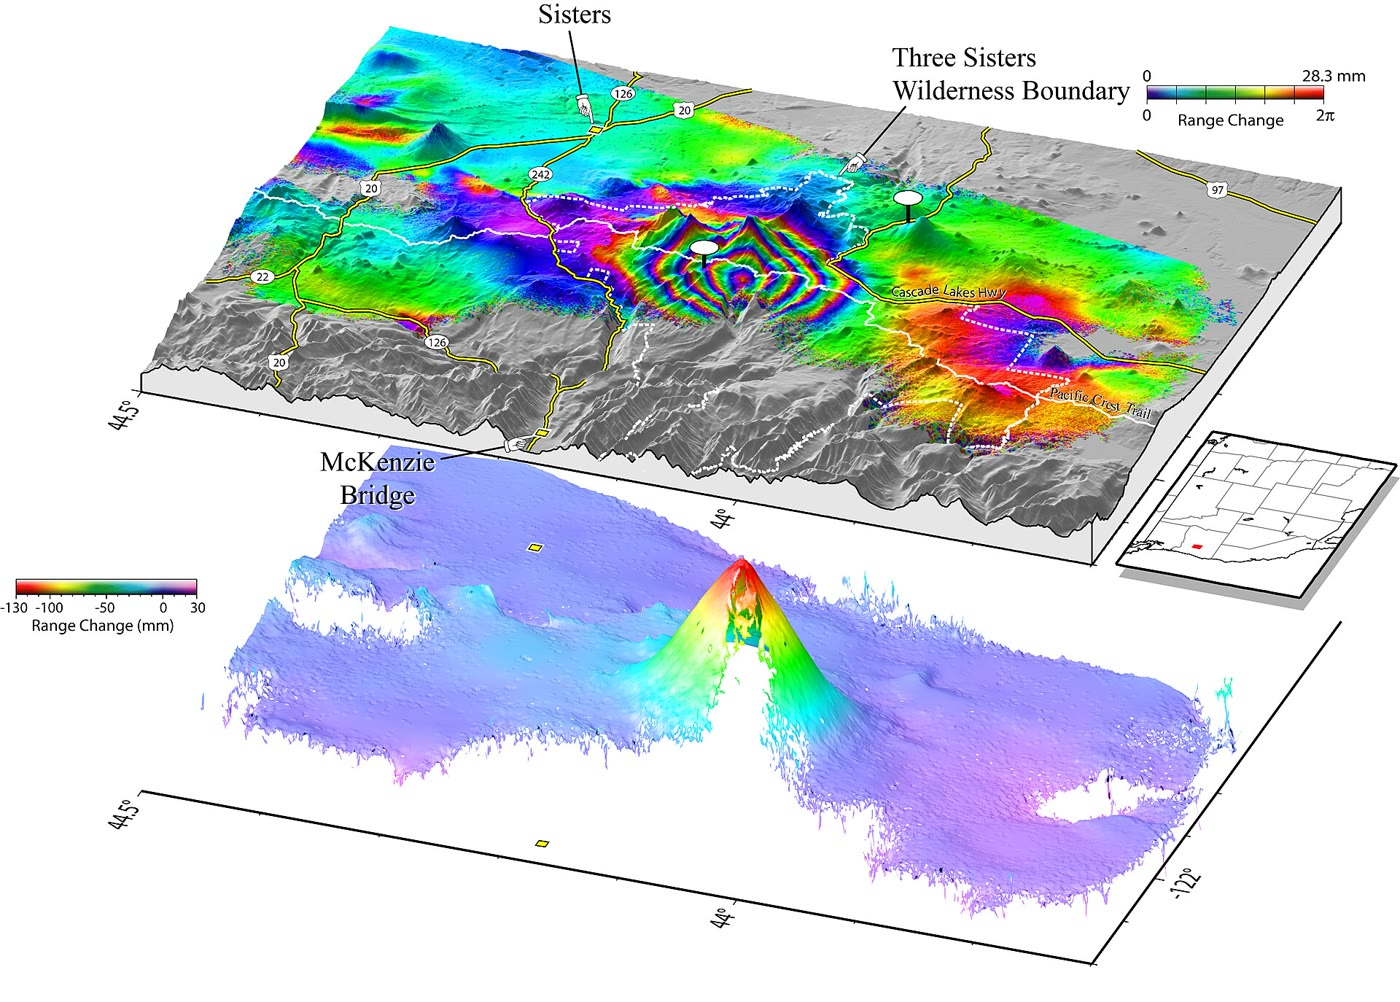
\includegraphics[width=0.86\linewidth]{images/book5/b3-three-sisters-insar.jpg}
\par\smallskip{\small أعلى، مخطّط التداخل لمركز الأخوات الثلاث
البركاني في أوريغون، 1995--2001، مُسقَطًا على التضاريس: كل دورة ألوان
تعادل \qty{28.3}{mm} من تغيّر المدى، وعين الثور المؤلَّفة من الحلقات
عند المركز تدلّ على الرفع. أسفل، البيانات نفسها بعد فكّ الالتفاف مرسومةً كتضاريس،
ويقصر المدى بمقدار يصل إلى \qty{130}{mm} عند المركز. الصورة:
\babelsublr{U.S. Geological Survey} (ويكس وآخرون، 2002)،
ملك عام.}\label{fig:b3:remote-sensing-gis:three-sisters}
\end{omfigure}
% ledger: photo:b3-three-sisters-insar, usgs:insar-fs

\begin{inthelab}[محطة أرضية]
\begin{minipage}[t]{0.55\linewidth}\vspace{0pt}
يسجّل قمر تصوير صناعي كمّيات تفوق بكثير ما يستطيع إرساله أثناء مروره
فوق المكان الذي يصوّره. يستطيع رادار القمر سنتينل-1 أن يصوّر
لمدّة تصل إلى نصف ساعة من كلّ مدار، ويخزّن بياناته على متنه، حتى
1410 غيغابت؛ ويرسلها إلى الأرض عبر قناتين بسرعة 260 ميغابت في الثانية لكلٍّ منهما،
فيستغرق إفراغ المخزن الكامل نحو 45 دقيقة.
تتلقّاها محطة أرضية: حين يطلع القمر فوق الأفق، يستدير الطبق ليتّجه نحوه،
يتتبّعه عبر السماء، ويتركه عند غروبه،
بينما يتحقّق المشغّلون من أنّ التدفّق يصل كاملًا. تنتقل البيانات بعد ذلك
إلى مركز معالجة تتحوّل فيه الأصداء الخام إلى صور.
\end{minipage}\hfill
\begin{minipage}[t]{0.42\linewidth}\vspace{0pt}
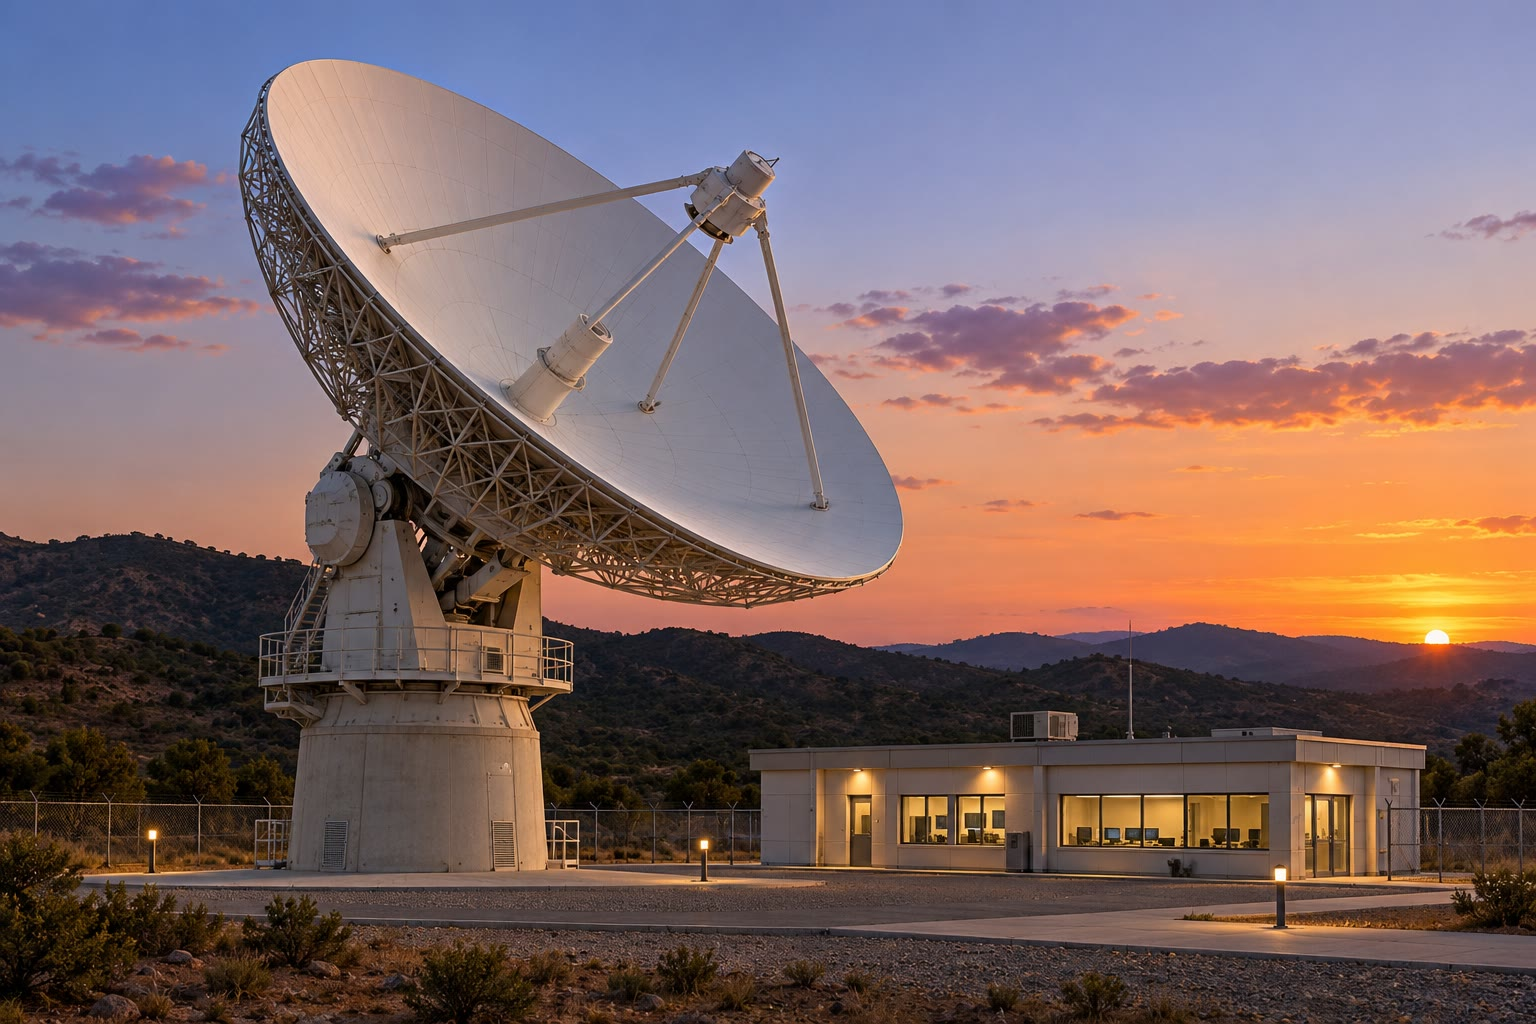
\includegraphics[width=\linewidth]{images/book5/ai/b3-ground-station.jpg}

{\scriptsize محطة أرضية لقمر صناعي عند الغسق: طبق تتبّع كبير ومبنى
عملياتها (رسم توضيحي مولَّد بالذكاء الاصطناعي).}
\end{minipage}
\end{inthelab}
% ledger: esa:s1-downlink

\section{نظم المعلومات الجغرافية}\label{sec:b3:remote-sensing-gis:gis}

تُعدّ صور الأقمار الصناعية، ونموذج الارتفاع الرقمي للأرض، والخريطة
الجيولوجية، والآبار، والطرق، طبقاتٍ لنظام معلومات جغرافي واحد،
يخزّنها في إطار إحداثي مشترك، ويُجري
عليها الحسابات.

\begin{definition}[البيانات الشبكية والبيانات المتجهية]\label{def:b3:remote-sensing-gis:data-models}
\emph{البيانات الشبكية}\index{البيانات الشبكية} تمثّل طبقةً بشبكة من
الخلايا، تحمل كلٌّ منها قيمةً واحدة: انعكاسيةً، أو ارتفاعًا، أو صنفًا.
\emph{البيانات المتجهية}\index{البيانات المتجهية} تمثّلها بنقاط وخطوط
ومضلّعات معطاة بإحداثيات رؤوسها، يحمل كلٌّ منها صفًّا من الخصائص
في جدول.
\end{definition}

\begin{omfigure}
\centering
\begin{tikzpicture}[x=0.5cm, y=0.5cm, font=\scriptsize]
\begin{scope}
\draw[black!40] (0,0) rectangle (10,7);
\fill[omSea!50, draw=omDef, thick] (3,4.5) ellipse (1.8 and 1.2);
\draw[omDef, very thick] (4.8,4.5) -- (7,3.5) -- (10,2);
\fill[red!70!black] (7,5.5) circle (0.14); \fill[red!70!black] (2,1.5) circle (0.14);
\node[anchor=south] at (5,7.1) {متجهة};
\node at (3,4.5) {بحيرة};
\node[anchor=south west] at (7.1,5.6) {\foreignlanguage{arabic}{بئر \mbox{\textdir TLT 1}}};
\node[anchor=south west] at (2.1,1.6) {\foreignlanguage{arabic}{بئر \mbox{\textdir TLT 2}}};
\node[anchor=north east] at (9.9,2.2) {النهر};
\end{scope}
\begin{scope}[xshift=6.5cm]
\foreach \i/\j in {1/4,2/4,3/4,4/4,2/3,3/3,2/5,3/5} {\fill[omSea!50] (\i,\j) rectangle ++(1,1);}
\foreach \i/\j in {5/4,6/3,7/3,8/2,9/2} {\fill[omDef!70] (\i,\j) rectangle ++(1,1);}
\foreach \i/\j in {7/5,2/1} {\fill[red!70!black] (\i,\j) rectangle ++(1,1);}
\draw[black!30, step=1] (0,0) grid (10,7);
\draw[black!40] (0,0) rectangle (10,7);
\node[anchor=south] at (5,7.1) {شبكية};
\end{scope}
\end{tikzpicture}
\par\smallskip{\small الخريطة نفسها ممثّلةً بيانات متجهة (يسارًا: مضلّع وخط
ونقطتان دقيقتان في موقعهما، ولكلٍّ منها خصائصه)، \omterm{def:b3:remote-sensing-gis:data-models}{وبيانات شبكية}
(يمينًا: قيمة واحدة لكلّ خلية، والبحيرة بالخلايا التي يقع مركزها داخلها،
والنهر والآبار بالخلايا التي تقطعها). يسهل الحساب بالشبكة خليةً خليةً،
أمّا الطبقة المتجهة فتحفظ الأشكال والطوبولوجيا عند
أيّ مقياس.}\label{fig:b3:remote-sensing-gis:raster-vector}
\end{omfigure}

\begin{definition}[الإسناد الجغرافي]\label{def:b3:remote-sensing-gis:georef}
\emph{الإسناد الجغرافي}\index{الإسناد الجغرافي} هو إسناد إحداثيات خريطة
ضمن إسقاط محدّد إلى كلّ بكسل في صورة، أو إلى كلّ رأس في رسم،
ويكون ذلك عادةً بملاءمة تحويل لنقاط الضبط الأرضية
التي تُعرف مواقعها في الحالتين.
\end{definition}

بالنسبة إلى شبكة موجَّهة نحو الشمال ضمن إطار إسقاطي، يكون التحويل تآلفيًّا:
تملك الخليةُ في العمود $i$ والصفّ $j$ ركنَها عند $E = E_0 + i\,\Delta$،
$N = N_0 - j\,\Delta$، حيث $\Delta$ حجمُ الخلية. وتُعاد عيّنةُ صورة القمر الصناعي
أوّلًا في شبكة من هذا النوع؛ وتُسقَط الطبقات ذات الإسقاطات المختلفة
إلى إسقاط واحد قبل جمعها.

\begin{method}[الميل والاتجاه والتظليل التضاريسي من نموذج الارتفاع الرقمي]\label{met:b3:remote-sensing-gis:slope}
على شبكة ارتفاعات $z_{i,j}$ ذات تباعد $\Delta$ ($i$ نحو الشرق، $j$
نحو الشمال)، نُقدّر التدرّج بالفروق المركزية،
\[
\frac{\partial z}{\partial x} \approx \frac{z_{i+1,j} - z_{i-1,j}}{2\Delta} ,
\qquad
\frac{\partial z}{\partial y} \approx \frac{z_{i,j+1} - z_{i,j-1}}{2\Delta} .
\]
\emph{الميل} هو $S = \arctan|\nabla z|$؛ و\emph{الاتجاه} هو
سمتُ أشدّ انحدار، أي اتجاه $-\nabla z$، $A =
\operatorname{atan2}(-\partial z/\partial x, -\partial z/\partial y)$
مقاسًا في اتجاه عقارب الساعة من الشمال. و\emph{التظليل التضاريسي} لضوءٍ آتٍ من
السمت $A_0$ عند زاوية سمت الرأس $Z$ هو $\cos Z\cos S + \sin Z\sin S
\cos(A_0 - A)$، أي جيب تمام الزاوية بين الضوء والعمودي
على سطح الأرض، ويُضبط على الصفر حيث يكون سالبًا.
\end{method}

الفرق المركزي دقيق لمستوٍ، ويكون خطؤه بمقدار
$\Delta^2 z'''/6$ في غير ذلك؛ والتظليل التضاريسي لتلال فاردن في مجلد السنة الأولى
حُسب بهذه الطريقة، مع إضاءة من الشمال الغربي.
تُضخّم المشتقّات أخطاء الشبكة: نموذجٌ فيه درجات بين صفوفه يُظهر
هذه الأخطاء على شكل خطوط في خريطة ميله.

\begin{definition}[جبر الخرائط]\label{def:b3:remote-sensing-gis:map-algebra}
\emph{جبر الخرائط}\index{جبر الخرائط} هو حساب طبقة شبكية جديدة
خليةً خليةً من طبقةٍ أو أكثر من الشبكة نفسها: بالعمليات الحسابية
(NDVI من نطاقين)، وبالمقارنة (الخلايا الأشدّ انحدارًا من
\ang{15})، وبالعمليات المنطقية (و، أو، لا)، أو من جوار
الخلية (الميل).
\end{definition}

\begin{definition}[النطاق العازل؛ التراكب]\label{def:b3:remote-sensing-gis:operations}
\emph{النطاق العازل}\index{النطاق العازل} لعنصر عند المسافة $d$ هو
المنطقةُ من الخريطة الواقعة ضمن $d$ منه. و\emph{التراكب}\index{التراكب}
يجمع طبقتين أو أكثر من المنطقة نفسها
في طبقة واحدة، ويحمل كلّ موضع من النتيجة خصائص الطبقات
كلّها؛ واختيار المواضع التي تستوفي عدّة شروط في آنٍ واحد
هو أكثر استعماله شيوعًا.
\end{definition}

\begin{omfigure}
\centering
\begin{tikzpicture}
\begin{groupplot}[group style={group size=2 by 2, horizontal sep=2.0cm, vertical sep=1.5cm},
  width=0.43\linewidth, axis equal image, enlargelimits=false,
  xmin=0, xmax=10, ymin=0, ymax=8,
  tick label style={font=\scriptsize}, label style={font=\small}, title style={font=\small}]
\nextgroupplot[title={(أ) الميل (بالدرجات)}, ylabel={الشمال \babelsublr{(km)}}, colormap/viridis,
  point meta min=0, point meta max=24, colorbar right,
  colorbar style={width=0.18cm, ytick={0,5,10,15,20}, tick label style={font=\tiny}, axis equal=false}]
\addplot[matrix plot*, mesh/cols=101, point meta=explicit] table[x=x, y=y, meta=slope] {figdata/out/bachelor-3-varden_gis-grid.dat};
\addplot[white, thick] table {figdata/out/shared-region-river.dat};
\nextgroupplot[title={(ب) الاتجاه},
  colormap={aspect}{rgb255=(220,20,30) rgb255=(240,200,0) rgb255=(30,170,60) rgb255=(30,90,220) rgb255=(220,20,30)},
  point meta min=0, point meta max=360, colorbar right,
  colorbar style={width=0.18cm, ytick={0,90,180,270,360}, yticklabels={\omnameCompassN,\omnameCompassE,\omnameCompassS,\omnameCompassW,\omnameCompassN}, tick label style={font=\tiny}, axis equal=false}]
\addplot[matrix plot*, mesh/cols=101, point meta=explicit] table[x=x, y=y, meta=aspect] {figdata/out/bachelor-3-varden_gis-grid.dat};
\addplot[black, thick] table {figdata/out/shared-region-river.dat};
\nextgroupplot[title={(ج) طبقتان}, xlabel={الشرق \babelsublr{(km)}}, ylabel={الشمال \babelsublr{(km)}},
  colormap={lay}{rgb255=(245,245,245) rgb255=(150,150,150) rgb255=(225,195,140) rgb255=(120,70,20)},
  colormap access=piecewise constant, point meta min=-0.5, point meta max=3.5,
  legend columns=2, legend style={font=\tiny, at={(0.5,-0.3)}, anchor=north, /tikz/every even column/.append style={column sep=4pt}}]
\addplot[matrix plot*, mesh/cols=101, point meta=explicit, forget plot] table[x=x, y=y, meta=layers] {figdata/out/bachelor-3-varden_gis-grid.dat};
\addplot[omDef, thick, forget plot] table {figdata/out/shared-region-river.dat};
\addlegendimage{area legend, fill={rgb,255:red,150;green,150;blue,150}, draw=black!40}
\addlegendentry{\foreignlanguage{arabic}{أشدّ انحدارًا من \mbox{\textdir TLT \ang{15}}}}
\addlegendimage{area legend, fill={rgb,255:red,225;green,195;blue,140}, draw=black!40}
\addlegendentry{الطَّفل}
\addlegendimage{area legend, fill={rgb,255:red,120;green,70;blue,20}, draw=black!40}
\addlegendentry{كلاهما}
\nextgroupplot[title={(د) التراكب}, xlabel={الشرق \babelsublr{(km)}},
  colormap={cls}{rgb255=(245,245,245) rgb255=(225,195,140) rgb255=(190,150,90) rgb255=(200,20,30)},
  colormap access=piecewise constant, point meta min=-0.5, point meta max=3.5,
  legend columns=2, legend style={font=\tiny, at={(0.5,-0.3)}, anchor=north, /tikz/every even column/.append style={column sep=4pt}}]
\addplot[matrix plot*, mesh/cols=101, point meta=explicit, forget plot] table[x=x, y=y, meta=class] {figdata/out/bachelor-3-varden_gis-grid.dat};
\addplot[omDef, thick, forget plot] table {figdata/out/shared-region-river.dat};
\addplot[black, thin, dashed, unbounded coords=jump] table[x=x, y=y] {figdata/out/bachelor-3-varden_gis-buffer.dat};
\addlegendentry{\foreignlanguage{arabic}{نطاق عازل بمسافة \mbox{\textdir TLT \qty{1}{km}}}}
\addlegendimage{area legend, fill={rgb,255:red,225;green,195;blue,140}, draw=black!40}
\addlegendentry{الطَّفل}
\addlegendimage{area legend, fill={rgb,255:red,190;green,150;blue,90}, draw=black!40}
\addlegendentry{الطَّفل داخل النطاق العازل}
\addlegendimage{area legend, fill={rgb,255:red,200;green,20;blue,30}, draw=black!40}
\addlegendentry{المحدّد}
\end{groupplot}
\end{tikzpicture}
\par\smallskip{\small جلسة نظم معلومات جغرافية على تلال فاردن، انطلاقًا من نموذج ارتفاعها
الرقمي على شبكة \qty{100}{m}. (أ)~الميل، ويبلغ \ang{23} على جانبي
الوادي؛ (ب)~الاتجاه، أي الجهة التي تواجهها الأرض، ويواجه جانبا
النهر أحدهما الآخر؛ (ج)~طبقتان: الخلايا الأشدّ انحدارًا من \ang{15}
وانكشاف الطَّفل الجوراسي؛ (د)~تراكبهما مع
\omterm{def:b3:remote-sensing-gis:operations}{النطاق العازل} \qty{1}{km} للنهر (المتقطّع): \qty{0.32}{km^2} من
الطَّفل الشديد الانحدار فوق النهر، وهي تصفية أولى لأرض قد
تنزلق.}\label{fig:b3:remote-sensing-gis:varden}
\end{omfigure}

يُنفّذ الشكل أعلاه السلسلة كاملةً: \omterm{def:b3:remote-sensing-gis:map-algebra}{جبر الخرائط} على شبكة الارتفاع
يعطي الميل والاتجاه؛ وتُحوِّل مقارنةٌ الميلَ إلى طبقة من الخلايا الشديدة الانحدار؛
والخريطة الجيولوجية تعطي الطَّفل؛ والنطاقُ العازل للنهر يعطي طبقةً ثالثةً؛
أمّا تقاطعها، وهو تراكب بالعامل المنطقي
\emph{AND}، فيُبقي 32 خليّةً من أصل 8181. والنتيجةُ لا تكون أجود من
الطبقات التي بُنيت عليها: فعلى شبكة أخشن تأتي الميول أخفّ انحدارًا، ويمرّ عدد أقلّ من الخلايا.

\begin{definition}[التصنيف الموجَّه؛ مصفوفة الالتباس]\label{def:b3:remote-sensing-gis:classification}
\emph{التصنيف الموجَّه}\index{التصنيف الموجَّه} إجراءٌ
يُسنِد كل بكسل في صورة إلى واحد من مجموعة من الأصناف، استنادًا إلى قواعد أو
إحصاءات مستخلصة من بكسلات تدريب يُعرف صنفها على الأرض.
و\emph{مصفوفة الالتباس}\index{مصفوفة الالتباس} تُحصي، لمجموعة منفصلة من بكسلات مرجعية،
كم بكسلًا من كلّ صنف حقيقي أُسند إلى كلّ صنف:
أي أنّ $n_{ij}$ بكسلًا صُنِّف على أنّه $i$ ينتمي في الحقيقة إلى $j$.
\end{definition}

يحوي القطرُ البكسلاتِ المصنَّفةَ تصنيفًا صحيحًا. ومع $N$ بكسلًا مرجعيًّا،
فتكون \emph{الدقّة الكلّية} هي $\sum_i n_{ii}/N$. أمّا \emph{دقّة المستخدِم}
لصنفٍ ما، أي $n_{ii}$ على مجموع صفّه، هي احتمال أن يكون البكسل
الذي تُسمّيه الخريطة $i$ فعلًا $i$؛ أمّا \emph{دقّة المنتِج}، أي $n_{ii}$
على مجموع عمودها، هي احتمال أن يكون $i$ الحقيقي قد خُرِّط بوصفه $i$.
يقارن معامل \emph{كابا} الدقّة الكلّية $p_o$ مع الدقّة
$p_e = \sum_i (\text{صفّ}_i)(\text{عمود}_i)/N^2$ التي يبلغها الإسناد العشوائي
بالمجاميع نفسها، فيكون: $\kappa = (p_o - p_e)/(1 -
p_e)$.

\begin{center}
\small
\begin{tabular}{l|ccc|c}
\hline
المصنَّف \textbackslash{} المرجع & ماء & غابة & صخر عارٍ & المجموع \\
\hline
ماء & 45 & 2 & 0 & 47 \\
غابة & 3 & 38 & 7 & 48 \\
صخر عارٍ & 0 & 5 & 30 & 35 \\
\hline
المجموع & 48 & 45 & 37 & 130 \\
\hline
\end{tabular}
\end{center}

في هذا المثال المصطنَع، يُصنَّف صحيحًا 113 من 130 بكسلًا، أي دقّة كلّية
تبلغ \qty{86.9}{\percent}. وللغابة دقّةُ مستخدِمٍ تساوي
$38/48 = \qty{79}{\percent}$ لكنّ دقّة المنتِج تساوي $38/45 =
\qty{84}{\percent}$: إذ صُنِّف سبعة بكسلات من الصخر العاري، ربّما في الظلّ، على أنّها غابة.
ويبلغ الإسناد العشوائي $p_e = 0.338$، فيكون $\kappa =
0.80$.

\section{التمارين}

\begin{exercise}[$\star$]\label{exo:b3:remote-sensing-gis:1}
لحقلٍ انعكاسيّتان قدرهما 0.06 في النطاق الأحمر و0.42 في
النطاق تحت الأحمر القريب لمصوِّر ما؛ ولقطعةِ أرضٍ محروثةٍ مجاورةٍ لها 0.21
و0.28. احسب NDVI للحقلين، وفسّر ما توحي به كلّ قيمة.
\end{exercise}

\begin{exercise}[$\star$]\label{exo:b3:remote-sensing-gis:2}
يغطّي مصوِّر لاندسات~8 شريطًا عرضه \qty{185}{km} ببكسلات قياسها \qty{30}{m}،
وقناتُه البانكروماتية ببكسلات قياسها \qty{15}{m}. (أ)~كم بكسلًا يحوي خطٌّ يعبر الشريط
في كلّ حالة؟ (ب)~كم مستوًى يعطي 12 بِتًّا، وكم مستوًى يعطي 8 بتّات؟
(ج)~ما \omterm{def:b3:remote-sensing-gis:resolutions}{زمن إعادة الزيارة} للمصوِّر لاندسات~8
وحده، ولمجموعة لاندسات 8 و9 معًا؟
\end{exercise}

\begin{exercise}[$\star$]\label{exo:b3:remote-sensing-gis:3}
(أ)~على مخطط تداخل سنتينل-1 ($\lambda = \qty{5.55}{cm}$) لحوضٍ يهبط،
تفصل ستّةُ أهداب الحافّةَ المستقرّة عن المركز.
ما التغيّر في خطّ النظر عند المركز؟ (ب)~ما قيمة هدّاب واحد
لقمرٍ أقدم طول موجته \qty{5.66}{cm}؟
\end{exercise}

\begin{exercise}[$\star$]\label{exo:b3:remote-sensing-gis:4}
يُحلِّق مقياس ارتفاع بالليزر على بُعد \qty{500}{km} فوق سطح الأرض. (أ)~كم من الوقت يستغرق نبضٌ
للعودة؟ (ب)~إذا ضُبط توقيت كلّ فوتون على \qty{800}{ps}، ما دقّة
مدًى واحدًا؟
\end{exercise}

\begin{exercise}[$\star\star$]\label{exo:b3:remote-sensing-gis:5}
بكسلٌ من نطاق~10 للمصوِّر لاندسات~8 (خُذ $\lambda = \qty{10.9}{\micro\metre}$)
يحمل، بعد \omterm{def:b3:remote-sensing-gis:atm-correction}{التصحيح الجوي}، شدّةً إشعاعيةً طيفيةً قدرها
\qty{9.0}{W.m^{-2}.sr^{-1}.\micro\metre^{-1}}. (أ)~احسب \omterm{def:b3:remote-sensing-gis:brightness}{درجة حرارة السطوع}
لهذا البكسل. (ب)~السطح حقل عشب انبعاثيّته 0.98:
ما درجة حرارته الحركية؟
\end{exercise}

\begin{exercise}[$\star\star$]\label{exo:b3:remote-sensing-gis:6}
يُحلّق رادار سنتينل-1 على ارتفاع \qty{693}{km} بهوائيٍّ طوله \qty{12.3}{m}
بطول موجة $\lambda = \qty{5.55}{cm}$. (أ)~مع إهمال انحناء
الأرض، احسب المدى المائل إلى نقطة تُرصد بزاوية سقوط
\ang{35}. (ب)~ما استبانة السمت التي يعطيها هوائيٌّ حقيقيّ بهذا الطول هناك،
وما الذي تعطيه الفتحة الاصطناعية؟ (ج)~ما طول
الفتحة الاصطناعية؟
\end{exercise}

\begin{exercise}[$\star\star$]\label{exo:b3:remote-sensing-gis:7}
نافذةٌ $3\times3$ من نموذج الارتفاع الرقمي بخلايا قياسها \qty{30}{m}
تُظهر القيم، والشمال في الأعلى،
\[
\begin{matrix} 412 & 418 & 425 \\ 405 & 410 & 418 \\ 398 & 401 & 409 \end{matrix}
\qquad (\unit{m}).
\]
باستخدام الفروق المركزية عند الخليّة المركزية، احسب الميل والاتجاه
وتظليل التضاريس، لضوءٍ قادم من الشمال الغربي يرتفع \ang{45} فوق
الأفق.
\end{exercise}

\begin{exercise}[$\star\star$]\label{exo:b3:remote-sensing-gis:8}
تُراجع خريطة الغطاء الأرضي على 160 بكسلًا مرجعيًا (الصفوف: الخريطة؛
الأعمدة: الواقع؛ الأصناف: ماء، غابة، محاصيل، مدينة):
\[
\begin{pmatrix} 48 & 3 & 1 & 0 \\ 4 & 37 & 6 & 1 \\ 2 & 5 & 29 & 2 \\ 0 & 1 & 2 & 19 \end{pmatrix} .
\]
احسب الدقّة الكلّية، ودقّة المستخدِم ودقّة المنتِج لكلّ
صنف، ومعامل كابا. أيّ الأصناف هو الأكثر إغفالًا؟
\end{exercise}

\begin{exercise}[$\star\star$]\label{exo:b3:remote-sensing-gis:9}
بكسل حراري قياسه \qty{100}{m} يحتوي على تدفّق حمم حديث عند \qty{1443}{K}
يغطّي منه \qty{4}{\percent}، وما تبقّى سطح أرضي عند \qty{290}{K}؛ ونعتبر
كليهما جسمًا أسود. (أ)~احسب \omterm{def:b3:remote-sensing-gis:brightness}{درجة حرارة السطوع} للبكسل
عند \qty{10.9}{\micro\metre} وقارنها بمتوسط درجة الحرارة.
(ب)~احسب نسبة الإشعاع الصادر عن الجسم الأسود للحمم وللأرض
عند \qty{2.2}{\micro\metre}، واحسب \omterm{def:b3:remote-sensing-gis:brightness}{درجة حرارة السطوع} للبكسل
عندها. أيّ حزمة ترصد الحمم بصورة أفضل؟
\end{exercise}

\begin{exercise}[$\star\star\star$]\label{exo:b3:remote-sensing-gis:10}
يُنشأ مخطّطان للتداخل يصفان التشوّه نفسه من مرورين، أحدهما
حين كان القمر شرق الأرض، والآخر حين كان غربها، وكلاهما عند
زاوية السقوط \ang{35}. وعند نقطة واحدة يتقلّص
\omterm{def:b3:remote-sensing-gis:insar}{خط النظر} بمقدار \qty{64}{mm} في الأول و\qty{38}{mm} في
الثاني. بافتراض عدم وجود حركة شمال--جنوب، احسب الإزاحة الشاقولية
والإزاحة نحو الشرق. لماذا لا يكفي مرور واحد؟
\end{exercise}

\begin{exercise}[$\star\star\star$]\label{exo:b3:remote-sensing-gis:11}
يفشل \omterm{def:b3:remote-sensing-gis:insar}{فكّ التفاف الطور} حيثما يقفز الطور بأكثر من $\pi$ بين
بكسلين متجاورين. (أ)~أثبت أنّ \omterm{def:b3:remote-sensing-gis:insar}{خط النظر} يجب أن يتغيّر بأقلّ من $\lambda/4$
من بكسل إلى الذي يليه، أي \qty{13.9}{mm} بالنسبة إلى سنتينل-1.
(ب)~لمصدر موغي عند $z_0 = \qty{4}{km}$ مع $\Delta V =
\qty{e7}{m^3}$ و$\nu = 0.25$، منظورًا إليه شاقوليًا، أثبت أنّ أشدّ
تدرّج للدالة $u_z$ يقع عند $r = z_0/2$، واحسبه. (ج)~ما أكبر
حجم للبكسل يُبقي الأهداب قابلة للتمييز؟
\end{exercise}

\begin{exercise}[$\star\star\star$]\label{exo:b3:remote-sensing-gis:12}
(أ)~أثبت أنّ NDVI يقع بين $-1$ و$+1$ من أجل انعكاسيّات غير سالبة،
وأنّه لا يتغيّر عند ضرب الانعكاسيّتين معًا بالعامل نفسه.
(ب)~للعشب انعكاسيّتان قيمتاهما 0.051 (أحمر)
و0.502 (تحت الحمراء القريبة). صورة غير مصحّحة تضيف إشعاع مسار
يعادل 0.03 في الأحمر و0.01 في تحت الحمراء القريبة. احسب
مؤشّر NDVI مع هذا الإشعاع ومن دونه. (ج)~ماذا يعني ذلك لخريطة
NDVI المُنشأة من صور غير مصحّحة في يوم ضبابي؟
\end{exercise}

\section{مسألة: جانب منتفخ على جبل هالفرين}

\begin{problem}[{مسألة نهاية الأسبوع --- الغطاء النباتي والحرارة ومخطّط
التداخل الراداري على بركان متخيَّل}]
\label{pb:b3:remote-sensing-gis:1}
جبل هالفرين، وهو بركان متخيَّل، قذف تدفّقات من الحمم في 1890 و1960
و2005 فوق منحدراته المُشجَّرة. يتصاعد البخار من حقل الفومارولات على قمّته.
تُعطى فيما يلي بيانات الأقمار الصناعية لسنة حديثة.

\medskip\noindent\textbf{الجزء الأول --- الغطاء النباتي على تدفّقات الحمم.} انعكاسيّات مصحّحة
في الحزمة الحمراء وحزمة تحت الحمراء القريبة:
\begin{center}
\small
\begin{tabular}{lcccc}
\hline
السطح & الغابة & تدفّق 1890 & تدفّق 1960 & تدفّق 2005 \\
\hline
الأحمر & 0.04 & 0.07 & 0.11 & 0.12 \\
تحت الحمراء القريبة & 0.38 & 0.30 & 0.21 & 0.14 \\
\hline
\end{tabular}
\end{center}
\begin{enumerate}
\item احسب NDVI للأسطح الأربعة.
\item رتّب التدفّقات حسب استعادة غطائها النباتي. هل الترتيب
  نفسه ترتيب أعمارها؟
\item لماذا لا يساوي NDVI لتدفّق 2005 الصفر، مع أنّه لا ينمو عليه
  شيء تقريبًا؟
\item لماذا يكون NDVI أكثر موثوقيّة من انعكاسيّة تحت الحمراء القريبة
  وحدها على منحدرات بركان شديدة الانحدار وغير متساوية الإضاءة؟
\end{enumerate}

\medskip\noindent\textbf{الجزء الثاني --- حقل الفومارولات.} في الحزمة الحرارية
(نأخذ $\lambda = \qty{10.9}{\micro\metre}$) الإشعاع المصحّح لبكسل
قياسه \qty{100}{m} في هضبة القمّة بعيدًا عن الفومارولات هو
\qty{8.40}{W.m^{-2}.sr^{-1}.\micro\metre^{-1}}، وإشعاع البكسل الواقع فوق
حقل الفومارولات \qty{9.95}{W.m^{-2}.sr^{-1}.\micro\metre^{-1}}.
\begin{enumerate}[resume]
\item احسب درجتي حرارة السطوع للبكسلين.
\item لصخر الهضبة انبعاثية تساوي 0.97. ما درجة حرارتها
  الحركية؟
\item فوهات الفومارولات والأرض الدافئة من حولها عند
  \qty{370}{K}. نعامل الفوهات وبقيّة البكسل أجسامًا سوداء،
  وما تبقّى عند إشعاع الهضبة، فما الكسر من البكسل الذي تغطّيه
  وما المساحة التي تشغلها؟
\item لماذا تقلّ متوسطة درجة الحرارة المرجَّحة بالمساحة للبكسل
  عن درجة حرارة سطوعه؟
\end{enumerate}

\medskip\noindent\textbf{الجزء الثالث --- مخطّط التداخل.} صورتان من سنتينل-1
($\lambda = \qty{5.55}{cm}$، زاوية السقوط \ang{35}، والقمر الصناعي شرق
الأرض) مأخوذتان بفارق 48 يومًا، وتُظهران نمط عين الثور على المنحدر الشرقي.
من منطقة مستقرّة إلى مركز النمط تُحصى خمسة أهداب كاملة وأربعة أعشار
من الهدب السادس، وكلّها في اتّجاه الحركة نحو
القمر الصناعي.
\begin{enumerate}[resume]
\item لماذا يجب أخذ الصورتين من الموضع نفسه تقريبًا، وكم
  دورة مدارية للقمر الصناعي الواحد تفصل بينهما؟
\item احسب تغيّر \omterm{def:b3:remote-sensing-gis:insar}{خط النظر} عند المركز.
\item عند المركز تتحرّك الأرض شاقوليًا فقط. احسب الرفع
  عنده.
\item فسّر لماذا لا يكون النمط دائريًا، وفي أيّ جانب تتكاثف الأهداب، شرقًا
  أم غربًا؟
\item على طول خط الشمال--الجنوب المارّ بالمركز، يتناقص تغيّر
  \omterm{def:b3:remote-sensing-gis:insar}{خط النظر} إلى نصف قيمته المركزية على بُعد \qty{3.4}{km} من
  المركز. لماذا يُستعمل هذا الخط، وما العمق الذي يعطيه لمصدر
  موغي؟
\item كم هدبًا يفصل المركز عن تلك النقطة ذات نصف الارتفاع؟
\item يمكن لبخار الماء في الجوّ أن يؤخّر أمواج الرادار بصورة مختلفة في
  التاريخين وأن يرسم أهدابًا خاصّة به. كيف يساعد مخطّط تداخل ثانٍ
  لزوج آخر من التاريخين على التمييز بين الأثرين؟
\end{enumerate}

\medskip\noindent\textbf{الجزء الرابع --- الحجم.} خذ $\nu = 0.25$.
\begin{enumerate}[resume]
\item انطلاقًا من $u_z(0) = (1 - \nu)\Delta V/(\pi z_0^2)$، احسب تغيّر
  حجم المصدر.
\item عبّر عنه بوصفه المعدّل المتوسط في اليوم وفي السنة خلال 48 يومًا.
\item احسب أكبر إزاحة أفقية وأين تحدث.
\item لو كان الخزّان كرةً نصف قطرها $z_0/3$، فكم سيكون
  حجمها، وما الكسر منه الذي يمثّله التغيّر؟
\item يغيّر الحجم المحدود لكرة نصف قطرها $z_0/3$ الرفع بنحو
  \qty{3}{\percent}. هل يغيّر ذلك إجابة السؤال~16
  تغييرًا ملحوظًا، بالنظر إلى دقّة عدّ الأهداب؟
\item ما الرصد الآخر، من الجزأين الأول والثاني أو من الأرض،
  الذي يدعم تفسير كون الخزّان في طور الامتلاء؟
\item أعطِ تغيّر حجم الخزّان تحت جبل هالفرين، بملايين
  الأمتار المكعّبة، بدقّة رقمين معنويّين.
\end{enumerate}
\end{problem}
% ledger: nasa:ndvi, esa:s1-sar, esa:s1-orbit, esa:s1-iw, dmodels:mogi, dmodels:mogi-radial, const:h, const:c, const:kB
